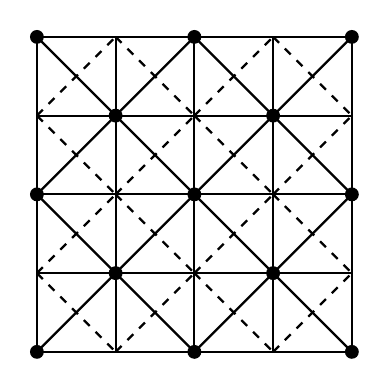
\begin{tikzpicture}[scale=1]
        % 绘制基础水平和垂直网格线
        \draw[step=1cm,black,thick] (0,0) grid (4,4);
        
        % 逐个小方格绘制对角线，避免实线和虚线重叠
        \foreach \x in {0,1,2,3} {
            \foreach \y in {0,1,2,3} {
                % 判断当前小方格左下角 (x,y) 坐标和的奇偶性
                \pgfmathparse{mod(\x+\y,2)==0}
                \ifnum\pgfmathresult=1
                    % 如果 (x,y) 是偶数点
                    % (x,y) 到 (x+1,y+1) 连结两个偶数点 -> 实线
                    \draw[thick] (\x,\y) -- (\x+1,\y+1);
                    % (x,y+1) 到 (x+1,y) 连结两个奇数点 -> 虚线
                    \draw[dashed,thick] (\x,\y+1) -- (\x+1,\y);
                \else
                    % 如果 (x,y) 是奇数点
                    % (x,y) 到 (x+1,y+1) 连结两个奇数点 -> 虚线
                    \draw[dashed,thick] (\x,\y) -- (\x+1,\y+1);
                    % (x,y+1) 到 (x+1,y) 连结两个偶数点 -> 实线
                    \draw[thick] (\x,\y+1) -- (\x+1,\y);
                \fi
            }
        }
        
        % 绘制节点（黑点和红星）
        \foreach \x in {0,1,2,3,4} {
            \foreach \y in {0,1,2,3,4} {
                \pgfmathparse{mod(\x+\y,2)==0}
                \ifnum\pgfmathresult=1
                    \fill[black] (\x,\y) circle (2.5pt);
                \else
                    % 使用略暗的红色以更贴近原图质感
                    \node[red!80!black] at (\x,\y) {\large $\bigstar$};
                \fi
            }
        }
    \end{tikzpicture}\par
    \vspace{0.5cm}
    
    % 图例部分
    \begin{tikzpicture}
        \fill[black] (0,0) circle (2.5pt) node[right=3pt, black] {偶数点};
        \node[red!80!black] at (2.5,0) {\large $\bigstar$};
        % 修正了图例中文字的颜色，原图文字为黑色
        \node[right=3pt, black] at (2.6,0) {奇数点};
    \end{tikzpicture}